\section{Our Work}
\subsection{Initial work}
\noindent
First, we downloaded the data and used the checksums.txt to validate. However,
there was one issue that downloading checksum.txt can also be distorted to
validate the data. After exploring the structure of data folder, we did some 
data fetching and preprocessing procedures. For behavior data, we wrote a 
function to merge three runs for each subject since we would like to look at 
the total observations within one subject. Also we noticed that in the data set
of each run, there existed observations with "-1" in "respcat", which was 
meaningless and might be an error during the experiment so we took them out.
For bold data, we also wrote a function to unzip all nii.gz files for further
analysis.

\subsection{Behavior Data}
\noindent
We did some explanatory data analysis and regression analysis using behavior 
data. For explanatory data analysis, we generated some summary statistics, 
including correlation among variables and simple plots to better understand 
the behavior. And then we used regression analysis to mainly answer two 
scientific questions. The scientific questions that we have are:
\begin{itemize}
\item If gain/loss would be significant for individuals who choose to 
participate and how much time it would take for them to respond.
\item If gain/loss would be significant for whether individuals would like to 
participate in the gamble. 
\end {itemize}

\subsubsection {Linear regression}
To answer the first question, we built three linear regression models.
\begin{enumerate}
\item  Response Time $\sim$ gain + loss
\item  Response Time $\sim$ diff(gain-loss)
\item  Response Time $\sim$ ratio(gain/loss)
\end {enumerate}
\textbf{Result} \\
We use the result for one subject to explain our findings. In the first model, 
p value for the predictor loss is 0.002644 while p value for the predictor gain 
is 0.547262. Basically, we can conclude that people would actually care more 
about loss than gain. In the second model, p value for the predictor difference
is 0.413985.  It turns out that we can conclude that the difference between gain 
and loss wouldn't be a factor for how much time it would take for a individual 
to respond. In the third model, p value for the predictor ratio is extremely 
small, showing that ratio has a huge impact on individuals' response time.

\subsubsection {Logistic regression}
\noindent
To answer the second question, we fit logistic regression between Accept/Reject
Gamble and gain/loss. According to our analysis, the decision to whether take 
the gamble of most of subjects, in general, is more affected by loss amount 
rather than by gain amount.  For example, below is the analysis on the subject 
3. The regression line shows that it well follows the border between the two 
decisions: 1 (gamble) and 0 (not gamble). Right side of the line illustrates 
the decision to not gamble and it takes up more area relative to the opposite 
decision.
\begin{figure}[H]
    \centering
        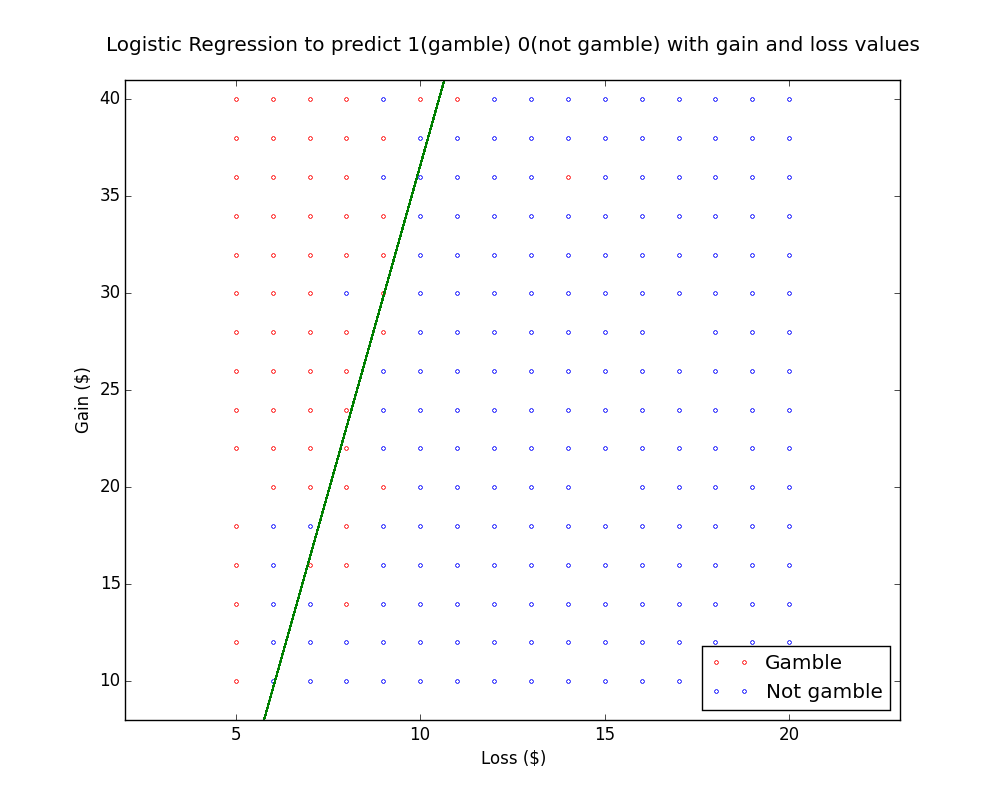
\includegraphics[scale=0.5]{log_regression.png}
    \caption{Logistic Regression for Subject 3}
\end{figure}


\subsection{BOLD data}
For image data, we did several explanatory data analysis to better under the 
BOLD data. 
\begin{itemize}
\item Reproduce Quality Assurance(QA) plots\\
 We reproduced some of the QA Plots provided in the BOLD folder, including 
 mean signals, Framewise Displacement and DVARS(root mean squared signal 
 derivative over brain mask). The shapes were almost the same, except the y 
 axis. We assumed there was some transformation or preprocessing in the 
 original QA plots.
\item Correlation \\
 We calculated the correlation between task-on/task-off vectors and voxel time 
 courses to identify the active region of the brain. Below is an example of correlation figure of the middle slice in subject 1.\\
  \begin{figure}[H]
    \centering
        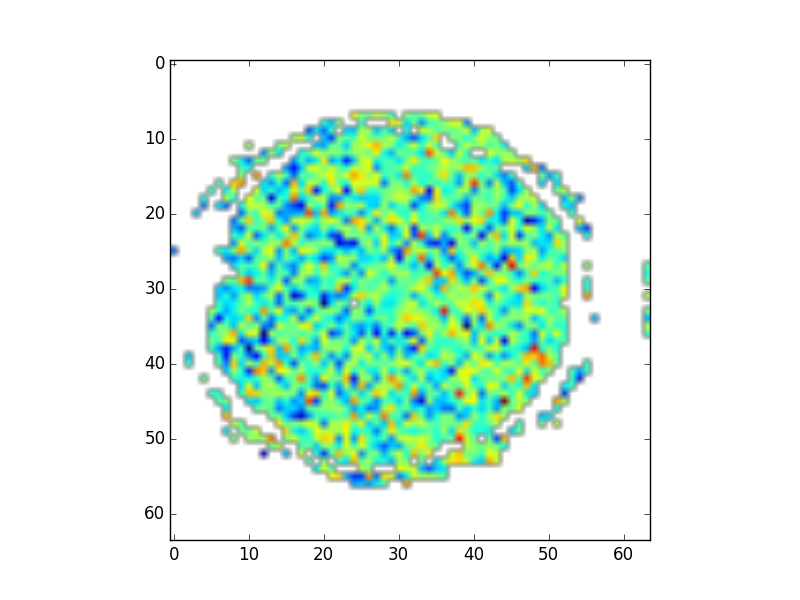
\includegraphics[scale=0.5]{correlations.png}
    \caption{Correlation between On/Off and Voxel Time Course}
\end{figure}
\item Associated the brain image data with behavior data\\
We started to associate brain image data(mean/standard deviation across time courses) with gain/loss/ratio, choices(accept/reject) and respcat(strongly/weekly accept/reject).
\end {itemize}